%
\chapter{Projeto A}

Quando começamos aprender uma nova linguagem, geralmente iniciamos com o exemplo mais básico, o \textit{"Hello Word"}. Nesse primeiro projeto, também vamos começar com a construção do \textit{"Hello Word"} da biblioteca MySensors e Pimatic, monitorando apenas a temperatura e umidade com um único nó sensor. Neste projeto, vamos construir um nó sensor simples com o intuito de monitorar a temperatura e umidade de uma sala. 

\section{Materiais}

Para esse projeto vamos o utilizar os seguintes materiais:
\begin{itemize}
\item 2 Arduinos;
\item Sensor de temperatura e umidade DTH11;
\item 2 Rádios RF;
\item Jumpers.
\end{itemize}

Para obter mais informações sobre os materiais consulte o capítulo ~\ref{MateSof}.

\section{Implementação}

Para a implementação desta atividade é necessário a construção dos seguintes nós.

\subsection{Gateway}

\vbox{
\indent \rule{10.4cm}{0.6pt}\par
\textbf{Esquemático}\par%\vspace{-0.66\baselineskip}
\rule[0.90\baselineskip]{10.4cm}{0.6pt}
}

\begin{figure}[ht]
      \centering
      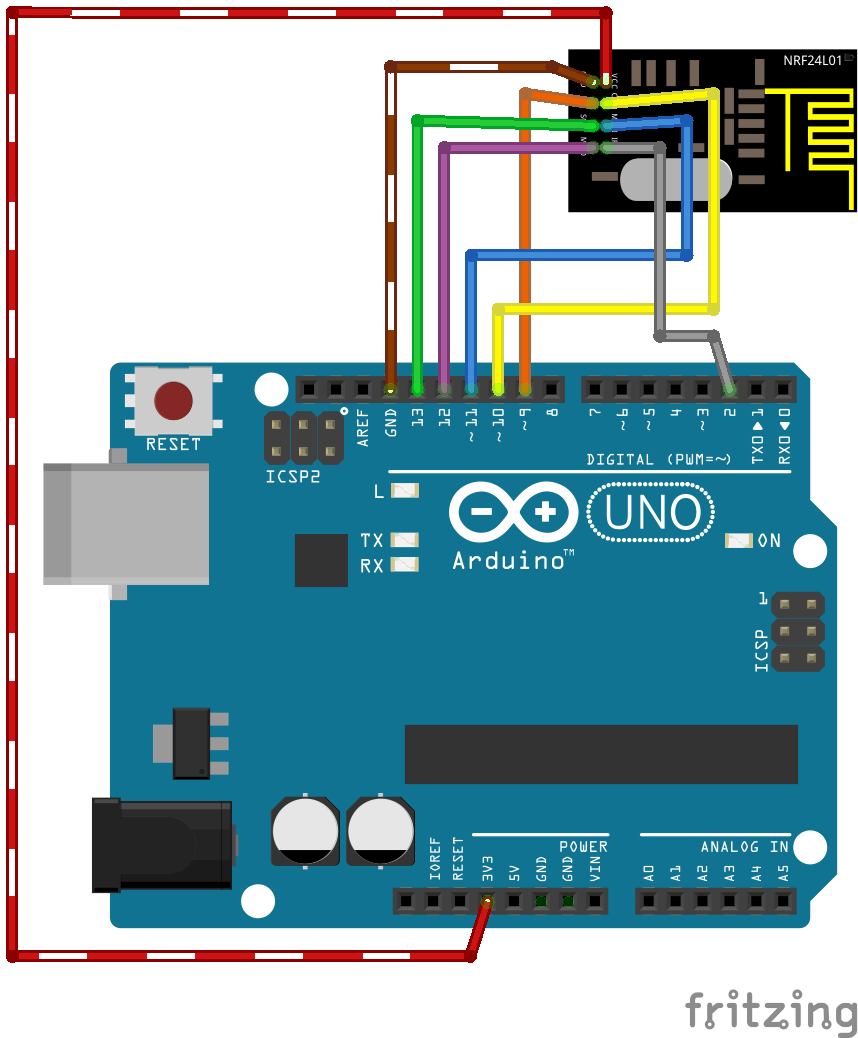
\includegraphics[scale=0.70]{figuras/gateway.png}
      \caption{Gateway}
      \label{fig:gateway}
\end{figure}
\pagebreak
\vbox{
\indent \rule{10.4cm}{0.6pt}\par
\textbf{Código}\par%\vspace{-0.66\baselineskip}
\rule[0.90\baselineskip]{10.4cm}{0.6pt}
}

\lstinputlisting[language=C++, caption={Gateway}]{code/teste.ino}

\subsection{Nó com sensor DTH11}

\vbox{
\indent \rule{10.4cm}{0.6pt}\par
\textbf{Esquemático}\par%\vspace{-0.66\baselineskip}
\rule[0.90\baselineskip]{10.4cm}{0.6pt}
}

\begin{figure}[ht]
      \centering
      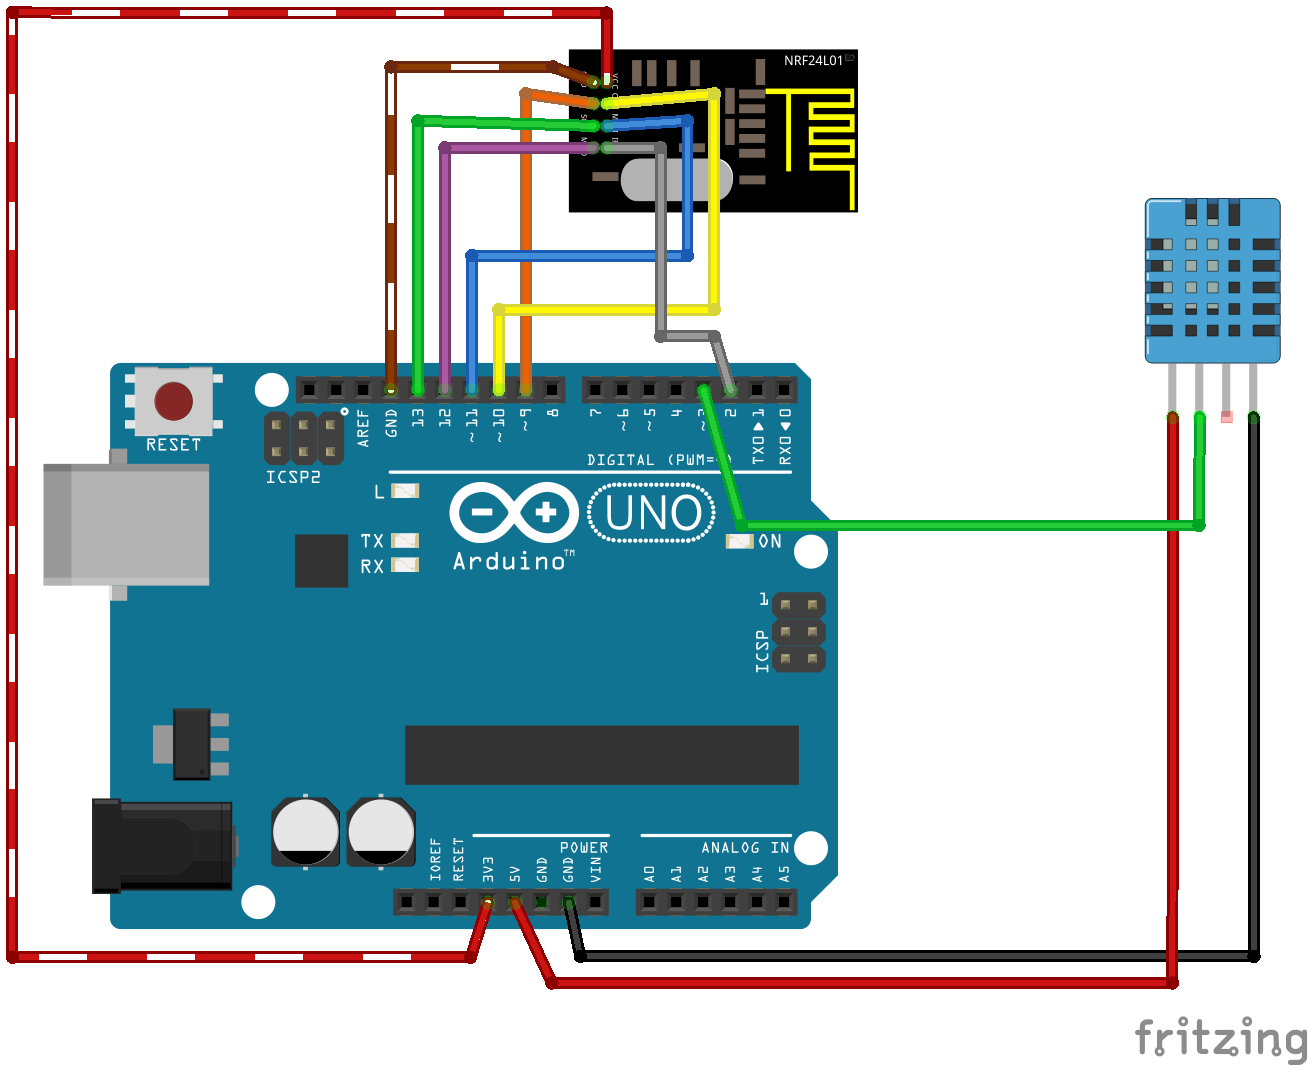
\includegraphics[scale=0.70]{figuras/DTH11_bb.png}
      \caption{Sensor DTH11}
      \label{fig:dth11}
\end{figure}
\pagebreak

\vbox{
\indent \rule{10.4cm}{0.6pt}\par
\textbf{Código}\par%\vspace{-0.66\baselineskip}
\rule[0.90\baselineskip]{10.4cm}{0.6pt}

}

\lstinputlisting[language=C++, caption={dth11}]{code/dth11.ino}


\subsection{Controlador}

Arquivo de configuração do Pimatic

\lstinputlisting[language=C++, caption={json.conf}]{code/jsonA.json}